% !TEX root = nips_2018.tex

\section{Soft Conditioning}\label{simmodels}

Conditioning on predicates requires a measure-theoretic foundation, in which a model is a collection of random variables:

\begin{figure}
	\centering
	\begin{minipage}[t]{0.5\linewidth}
		\centering
		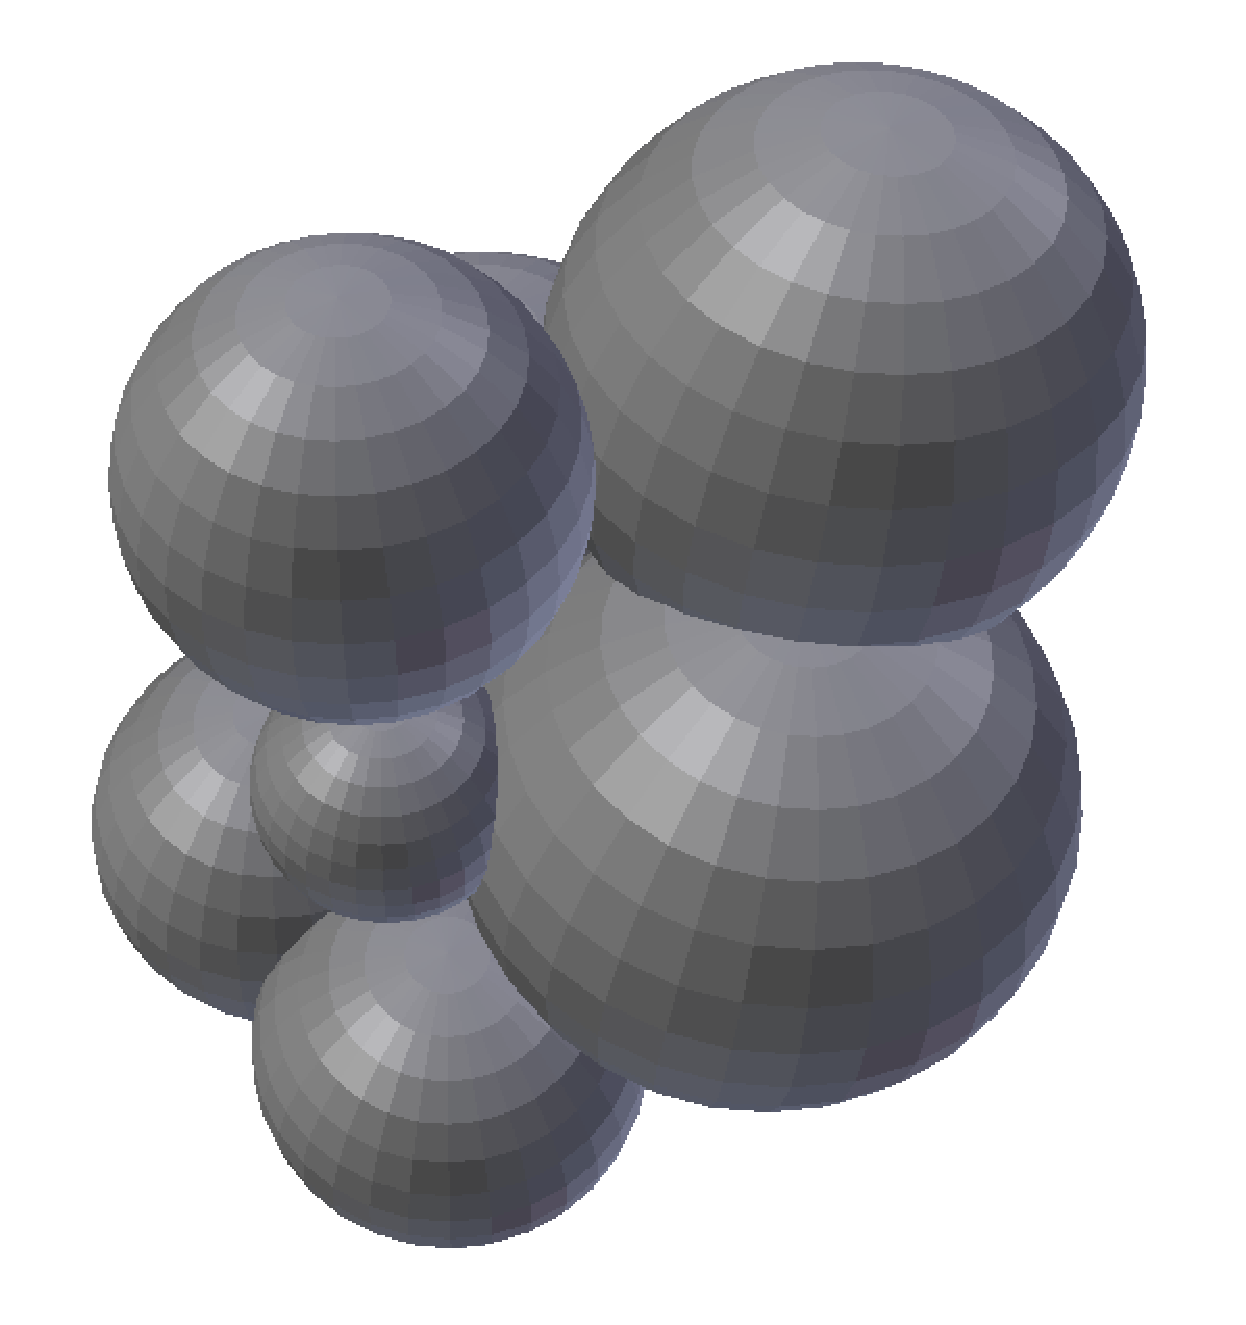
\includegraphics[width=0.8\linewidth]{clunk.eps}
	\end{minipage}%
	\begin{minipage}[t]{0.5\linewidth}
		\centering
		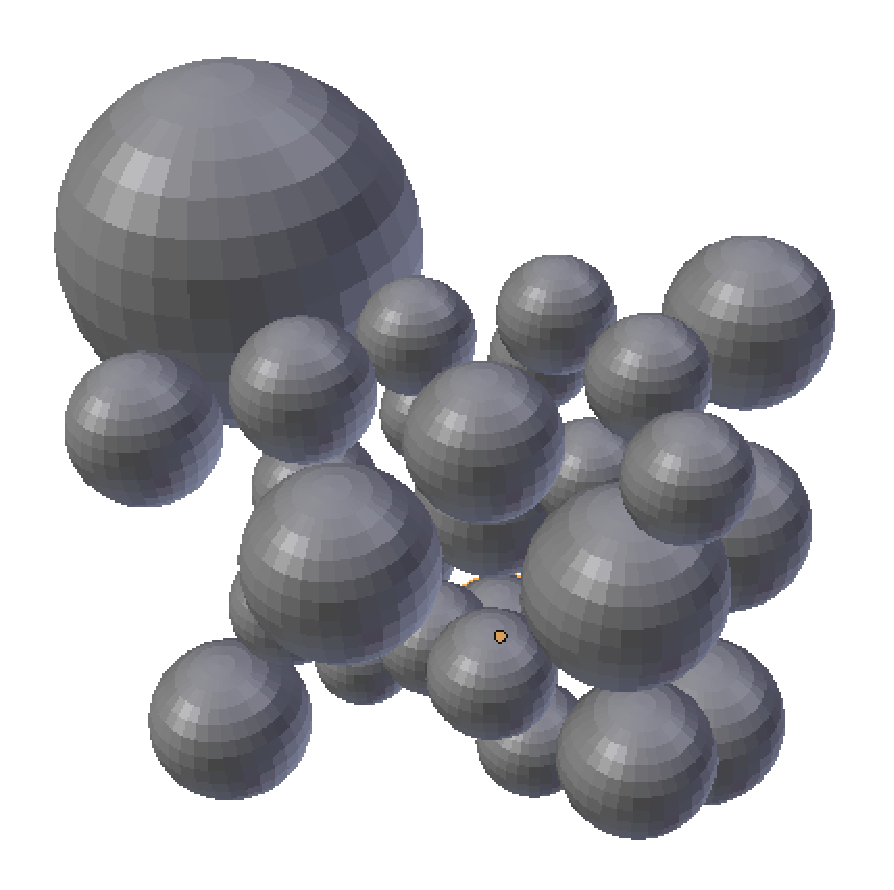
\includegraphics[width=0.8\linewidth]{nointersect.eps}
	\end{minipage}%
	\caption{Sample from geometric prior (left), whereas (right) is conditioned on no-intersection constraint}
	\label{fig:nointersect}
\end{figure}


\paragraph{Random Variables.} Probability models lie on top of probability
spaces. A probability space is a measure space $(\Omega, {\cal H}, {\cal P})$,
where ${\cal H}$ is a sigma algebra and ${\cal P}(\Omega) = 1$ \citep{ccinlar2011probability}. Random variables are
functions from the space $\Omega$ to a realization space ${\cal X}$. For example, if ${\cal P}$ is a uniform measure over subsets of the unit interval $\Omega$, a normal random variable $\Omega \to \mathbb{R}$ is the inverse cumulative distribution function of the normal.

\paragraph{Model} A \emph{model} $\cM$ is a collection of random variables along with a probability space.
% To fully specify a model, we need both the measure space and the
% collection of random variables on which it acts.

\paragraph{Conditioning}

Conditioning a model creates a new model.
As an example consider a model $\cM$ with two
random variables $X_1$ and $X_2$ that both take real values. Conditioning
$\cM$ on $X_1 = 1$, defines a new model $\cM_{|A}$ based on limiting the measure space
$\Omega$ to the set $A = \{ \omega : X_1(\omega) = 1\}$.
The new model is defined on a new probability space
\begin{align}\label{eq:condhard}
	(\Omega \cap A, \{A \cap B, B \in {\cal H} \}, {\cal P} / {\cal P}(A))
\end{align}
with the same random variables $X_1$ and $X_2$.
Sampling from $\cM_{|A}$ produces
samples only where $X_1 = 1$

More generally, conditioning on any predicate $Y(\omega) = \lk(X_1(\omega), \dots, X_n(\omega))$
defines a new model defined exactly as above, where $A = \{\omega : \lk(X_1(\omega), \dots, X_n(\omega)) = 1\}$.
% This predicate may include a comparisonsuch as $X_i < X_j$, restrict deterministic function of variables in in the model such as $\exp(X_i) = 2$, or be a Boolean combination such as $(X_i < X_j) \lor \neg(\exp(X_i) = 2)$.
Sampling from $\cM_{|A}$ generates $(x_1, ..., x_n)$ where $\lk$ is true.

% The general construction of new models might require conditioning
% on sets of measure zero. This process can be made rigorous
% via disintegration \citep{chang1997conditioning}. Disintegration can
% be thought of as the reversal of building joint distributions through
% product measure constructions.

\paragraph{Soft Conditioning}
Rather than a restriction of a probability space to an event, we can define conditioning as a transformation of a measure.

\begin{definition}Let $(\Omega, \mathcal{H}, \mathcal{P})$ be a measure space.
Soft conditioning on a function $Y: \Omega \to [0, 1]$ constructs a new measure $\mathcal{P}'$ defined as:
\begin{equation}\label{eq:softcond}
\mathcal{P}'(A) = \frac{E(1_A\softv{Y})}{E(\softv{Y})}
\end{equation}

If $Y$ is a predicate, i.e. an indicator function defined on $[0, 1]$ then Equation \ref{eq:softcond} is equivalent to hard conditioning on events (Equation \ref{eq:condhard}).
\end{definition}


% When building models with prior beliefs via conditioning, we would like
% the property that given an infinite collection of observations, the 
% posterior predictive distribution converges to true sampling distribution.
% To study this, consider a model with two random variables that are independent,
% $X_1$ is a function of $\omega_1$ and $X_2$ is a function of $\omega_2$. Suppose
% that the true sampling distribution has $X_1$ and $X_2$ positively correlated.
% For the prior beliefs to support positive correlations, we 
% could condition on a prior belief that $X_1$ and $X_2$ are close. However
% if the form of the closeness isn't controlled by a random variable, observing
% an arbitrary amount of data from the true distribution will not change
% the dependence between $X_1$ and $X_2$ in the model. 
% \begin{align*}
% X_j^*(\omega^*) = \sigma(f_\Beta(X_{j, 1}, ..., X_{j, n})) > b, \\
% \end{align*}
% Conditioning on $X_j^*$ produces a new set of models that have 
% dependence between . Knowledge is encoded in the prior distribution
% on $\Beta$. If $f_\Beta$ has priors over the true dependence between
% $X_{., 1},...,X_{., m}$, then this new model family will converge
% to the true underlying distribution.

% rr: TODO the above can me made into a proof

% \subsection{Bayesianism vs. Bayesian Computation}
% The way we 


% \section{Higher Order Random Variables}
% People often entertain beliefs about probability statements. For instance most people accept 
% trust expert-given odds that a particular sports team will win a tournament, 
% or politician will win an election, more than the odds of those given by non-experts.
% The apparent failure of probabilistic expressions to distinguish 
% between these cases led to alternative formalisms of uncertainty \citet{Shampher}, 
% but within the probabilistic framework both \citet{Pearl} and \citet{Hyberg} demonstrated 
% that such higher order distributions were induced from the original model, no new machinery was needed.

% As a concrete example of this, suppose we have a stochastic 
% dynamical system model of human blood glucose 
% controlled by some 
% parameters $\Theta$ with a prior. A priori we know that the average blood pressure 
% in a person lives in a physically plausible range $40-400$. A way to
% encode this would be to change the prior on the parameters $p(\Theta)$ 
% to so that any sample from that prior yields has average in the physically
% plausible range. This can be challenging because it requires a detailed
% understanding of the stochastic dynamical system. 

% Alternatively, we could try to take the conditioning approach from the
% previous section. But conditioning in the previous section required explicitly
% defined random variables, and while the average glucose is a random variable
% because the parameter $\Theta$ is random, it is not an explicit random variable.
% The scenario requires the ability to both define and condition on 
% probability distributions over either random variables or properties of 
% random variables (e.g. expectations).
% In this section we introduce the random conditional 
% distribution ($\randcond$) to support this task.

% \paragraph{The Random Conditional Distribution.}
% The random conditional distribution of $X$ given $\Theta$ -- which we denote $\rcd(X, \Theta)$ or $\rcdxy{X}{\Theta}$ -- is a random distribution: a random variable which takes values in the domain of random variables.
% Informally, $\rcdxy{X}{\Theta}$ is a function of $\omega$ that returns functions of $\omega$
% of the same type as $X$. Formally, $\rcd$ is a distribution over conditional random variables:

% % The primary mechanism for conditioning is $\cond$, which constructs conditional random variables:
% % \begin{definition}
% % Let $X:\Omega \to T$ be a random variable, $Y$ an indicator function, and $\conds{X}{Y}: \Omega_{|Y} \to T$ be a conditional random variable defined as: $X_{|Y}(\omega) = X(\omega)$.
% % $X_{|Y}$ is defined on a conditioned probability space $(\Omega, \Sigma, \mu_{|Y})$ where $\mu_{|Y}$ is a conditional measure: $
% % \mu_{|Y}(A) = \mu(A \cup Y^{-1}(\{1\})) / \mu(Y^{-1}(\{1\})$.
% % % That is, $\cond: (\Omega \to T) \times (\Omega \to \{0, 1\}) \to (\Omega \to T)$ is a operator that restricts the domain of $X$ to those inputs consistent with $Y$.
% % \end{definition}


% \begin{definition}The random conditional distribution of a random variable $X: \Omega \to T_1$ given $\Theta: \Omega \to T_2$ is a random variable $\rcdxy{X}{\Theta}: \Omega \to (\Omega \to T_1)$, defined as:
% \begin{equation}\label{eq:rcd}
% (\rcdxy{X}{\Theta})(\omega) = [\conds{X}{\Theta = \Theta(\omega)}]
% \end{equation}
% \end{definition}
% For example if $\Theta = \bern(0.4)$ and $X = \normal(\Theta, 1)$, then $\rcdxy{X}{\Theta}$ is a random distribution 
% whose domain comprises of two normal distributions $X_1 = \conds{\normal(\Theta, 1)}{\Theta = 1}$ and $X_2$.
% The probabilities of $X_1$ and $X_2$ with respect $\rcdxy{X}{\Theta}$ are determined by the prior probabilities of the different outcomes of $\Theta$: $P((\rcdxy{X}{\Theta}) = X_1) = 0.4$ and $P((\rcdxy{X}{\Theta}) = X_2) = 0.6$.

% A random conditional distribution is most useful in combination with other functions.
% Expectation is perhaps the most important example, which when composed with $\rcd$ produces conditional expectation.
% Restricting to real valued variables, expectation $E$ is a functional that maps a random variable to a real value
% (($\Omega \to \mathbb{R}) \to \mathbb{R}$).
% When $X$ is a real valued random variable, $\rcdxy{X}{\Theta}$ is not real valued, and hence not a valid argument to $E$.

% However, just as arithmetic operations such as $+$ and $-$ extend from the domain of numbers to the domain of random variable (pointwise $X + Y = \omega \mapsto X(\omega) + Y(\omega)$), $E$ extends from the domain of random variables to the domain of random variables over random variables in precisely the same way.
% % Since random variables are themselves functions, $E$ is an operator, functional or more generally a higher-order function.  
% % As described in section X a function with domain $T$ can be lifted to a functional of $T$-valued random variables.
% % $T$ is purposefully left abstract, because in addition to lifting functions defined on the reals etc, we can lift functions defined on random variables.
% % Expectation is a cannonical example of a random variable valued function, with type $E : (\Omega \to \mathbb{R}) \to \mathbb{R}$.
% That is, $\ee$ has a lifted counterpart $\lifted{\ee} = \lift(\ee)$ with type $\lifted{\ee} : (\Omega \to (\Omega \to \mathbb{R})) \to (\Omega \to \mathbb{R})$, which maps a distribution over real valued random variables to a distribution over real values (expectations).
% % $$
% % \lifted{\ee}(X)(\omega) = \mean{X(\omega)}
% % $$
% The operator $\rcd$ composed with $\ee$ constructs conditional expectation (with respect to a random variable $\Theta$):
% \begin{equation}
% \lmean{\rcdxy{X}{\Theta}} = \lmean{\omega \mapsto \conds{X}{\Theta = \Theta(\omega)}} 
%                     = \omega \mapsto \mean{\conds{X}{\Theta = \Theta(\omega)}}\\
% \end{equation}
% The final term $\omega \mapsto \mean{\conds{X}{\Theta = \Theta(\omega)}}$ matches the definition of
% conditional expectation
% with respect to a random variable $\mean{(X\mid \sigma (Y))(\omega)} = \mean{X \mid Y = Y(\omega))}$.
% That is the conditional expectation is a random variable with randomness provided by the conditioning set.

% Returning to the blood glucose example, we can build a model that respects the valid range
% of average blood glucose by taking the original model creating the conditional expected
% value of glucose $G$ with $\rcd$ and expectation of $\rcd$, then constructing a new model
% by conditioning the original on $G$ being in the physiologically possible range.

% \paragraph{Completeness.}Nested uses of $\rcd$ lead to a completeness result. State informally: 
% by repeatedly applying $\rcd$, any random function or functional in the original model
% can be constructed. Then by using conditioning to create new models from the previous 
% section, we can alter existing models to respect predicates on any random quantity in
% the model even if the random quantity is not an explicit random variable.
% % RR: TODO: The above could be a theorem

